\section{Middlebox Recovery without Rolling Back}

On contrary to FTMB, we aim to provide a new middlebox replication strategy
which keeps both the primary and the backup instances in synchronization. This
replication strategy directly gives the same input packet stream to both the
primary instance and the backup instance, our new architecture is able to keep
both of the two instances in synchronization.

Using this strategy, there is no need to roll-back the backup instance when the
primary instance fails. This strategy minimizes the recovery time and eliminates
the prolonged packet processing delay when checkpointing the primary instance.

To tackle the challenge of keeping both the primary instance and the backup
instance in synchronization, one might resolve to deterministic scheduling
\cite{}. However, the overhead caused by deterministic scheduling is way too
high for NF software, as a typical NF software needs to process millions of
input packets every second. Instead, we solve the deterministic execution
problem using a combination of coroutine and message passing.

\begin{verbbox} Temporarily removed. \end{verbbox}

\begin{figure}[!t]
  \begin{subfigure}[t]{0.5\linewidth}
    \centering
    %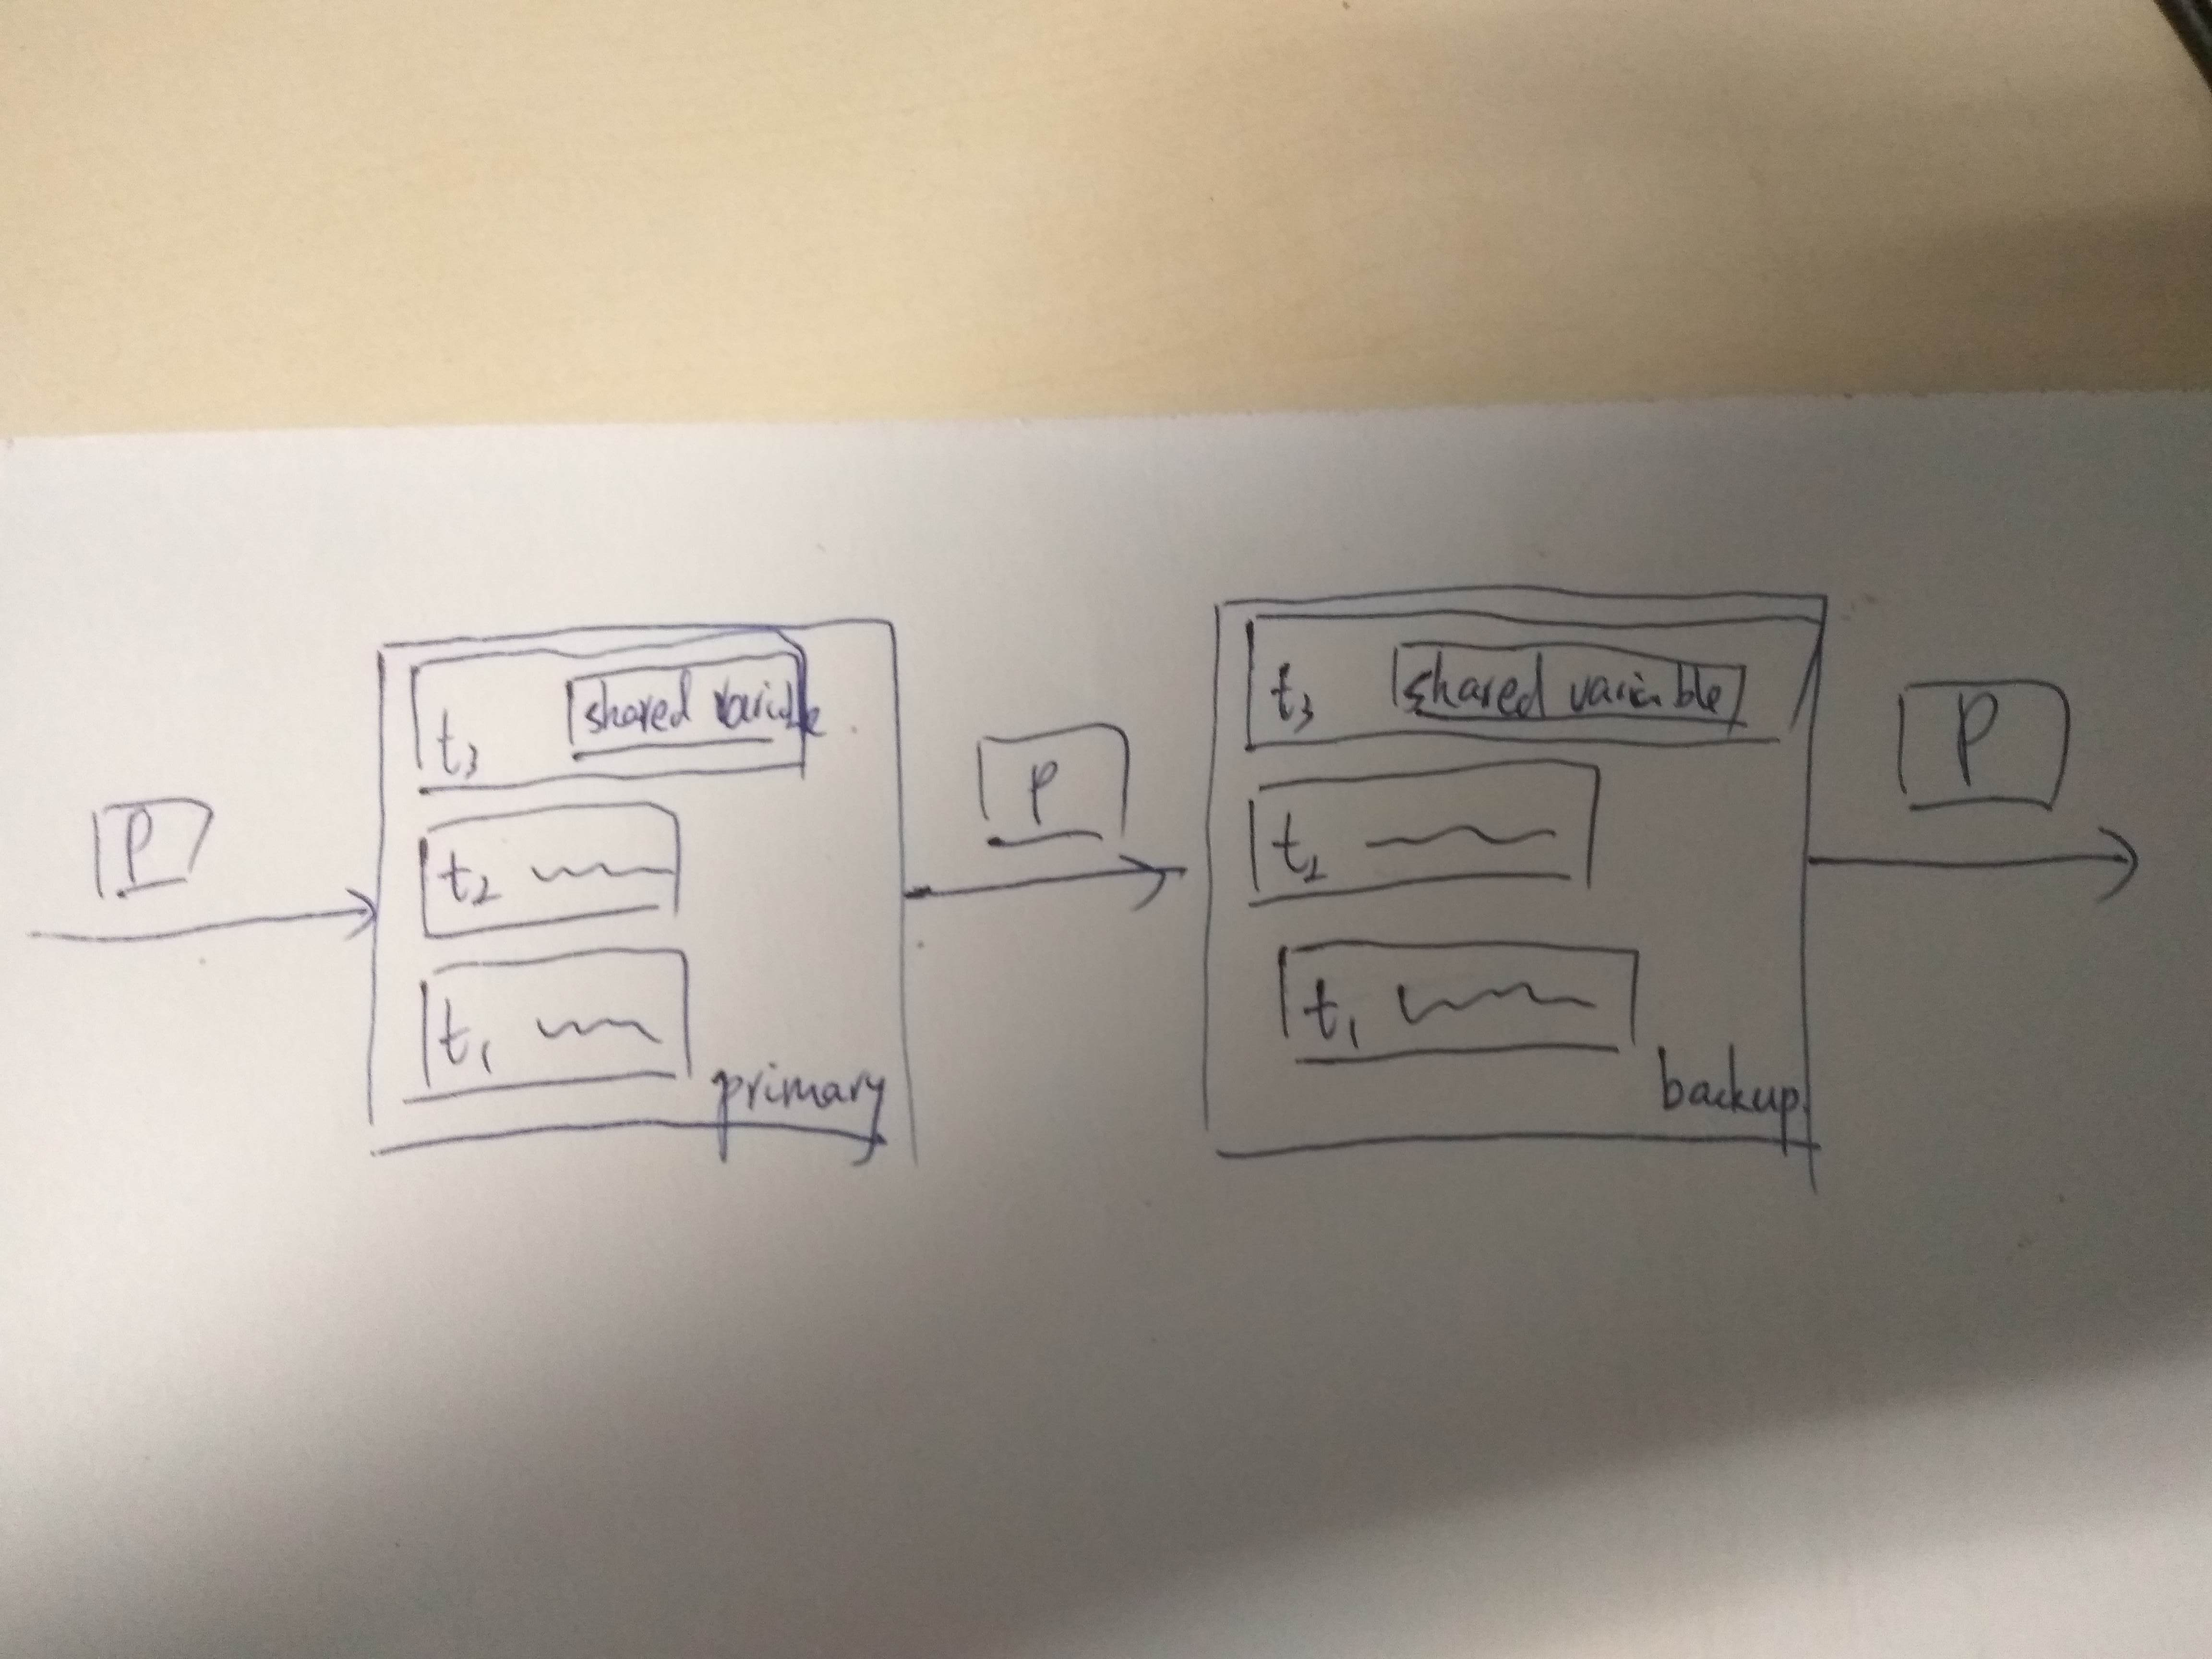
\includegraphics[width=\columnwidth]{section/overall.jpg}
    \resizebox{0.95\columnwidth}{!}{\theverbbox}
    \caption{The basic setup.}\label{fig:overall}
  \end{subfigure}\hfill
  \begin{subfigure}[t]{0.5\linewidth}
    \centering
    %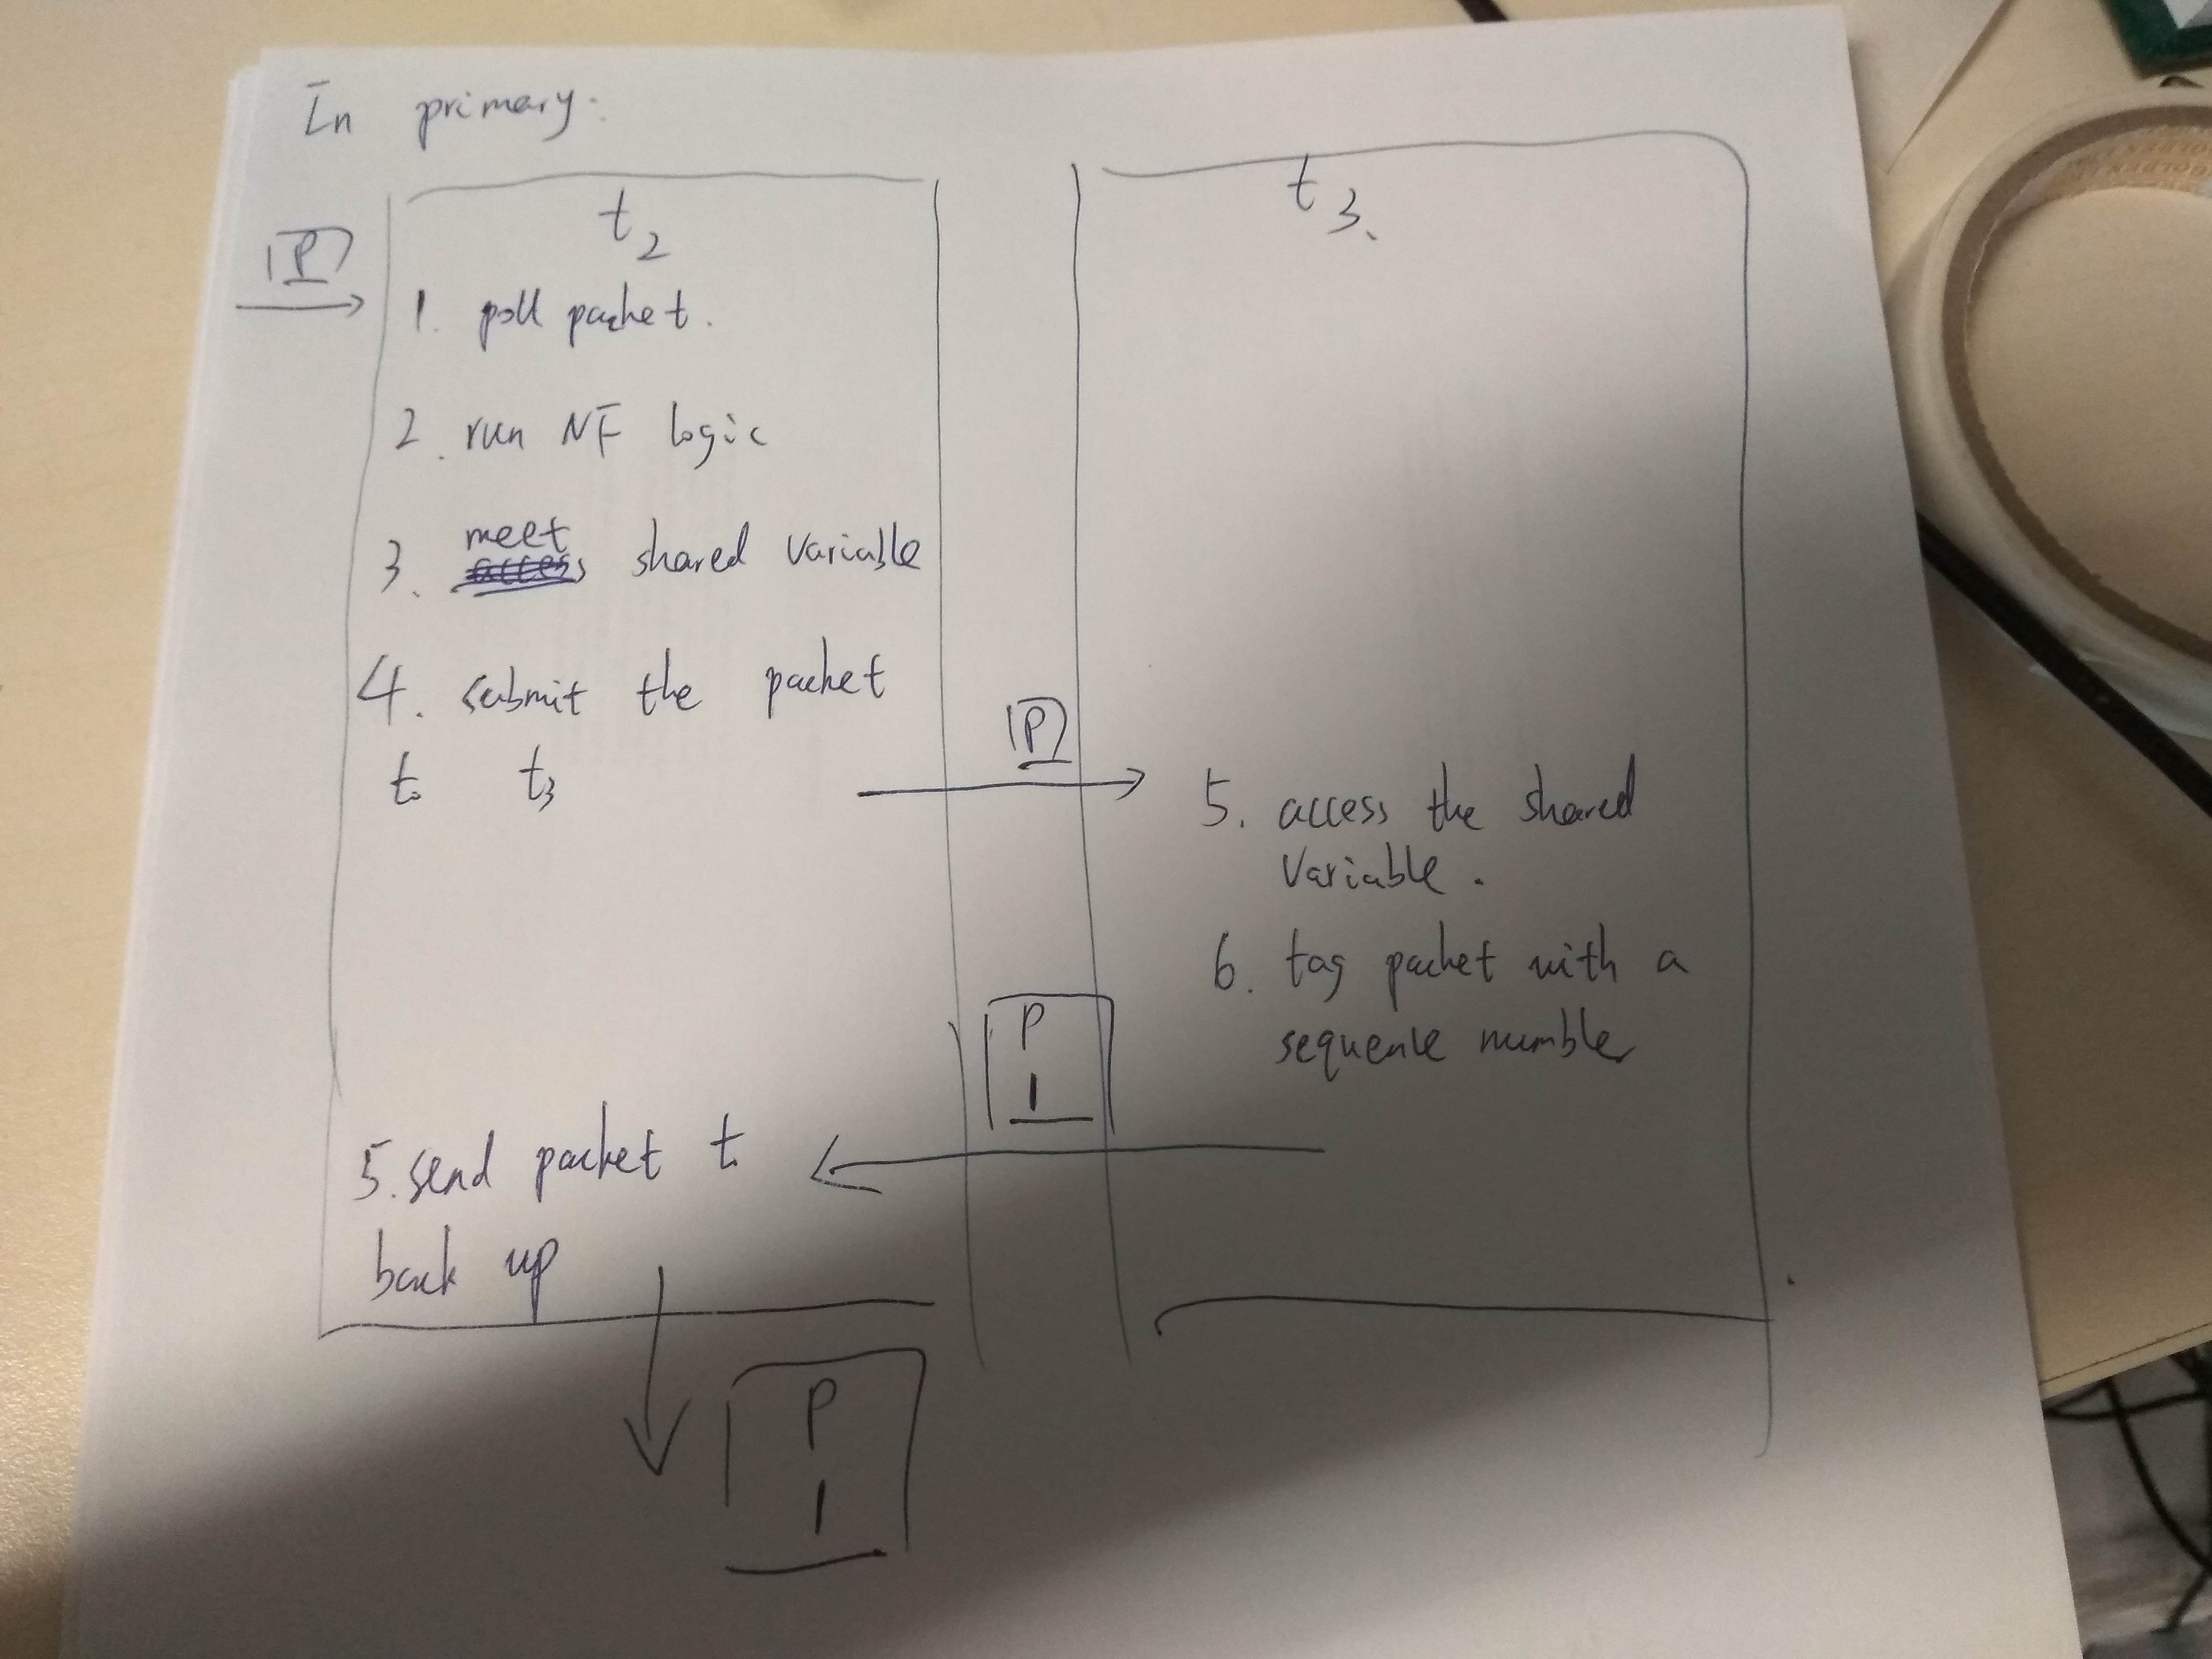
\includegraphics[width=\columnwidth]{section/primary.jpg}
    \resizebox{0.95\columnwidth}{!}{\theverbbox}
    \caption{The execution flow on a primary instance.}\label{fig:primary}
  \end{subfigure}\hfill
  \begin{subfigure}[t]{0.5\linewidth}
    \centering
    %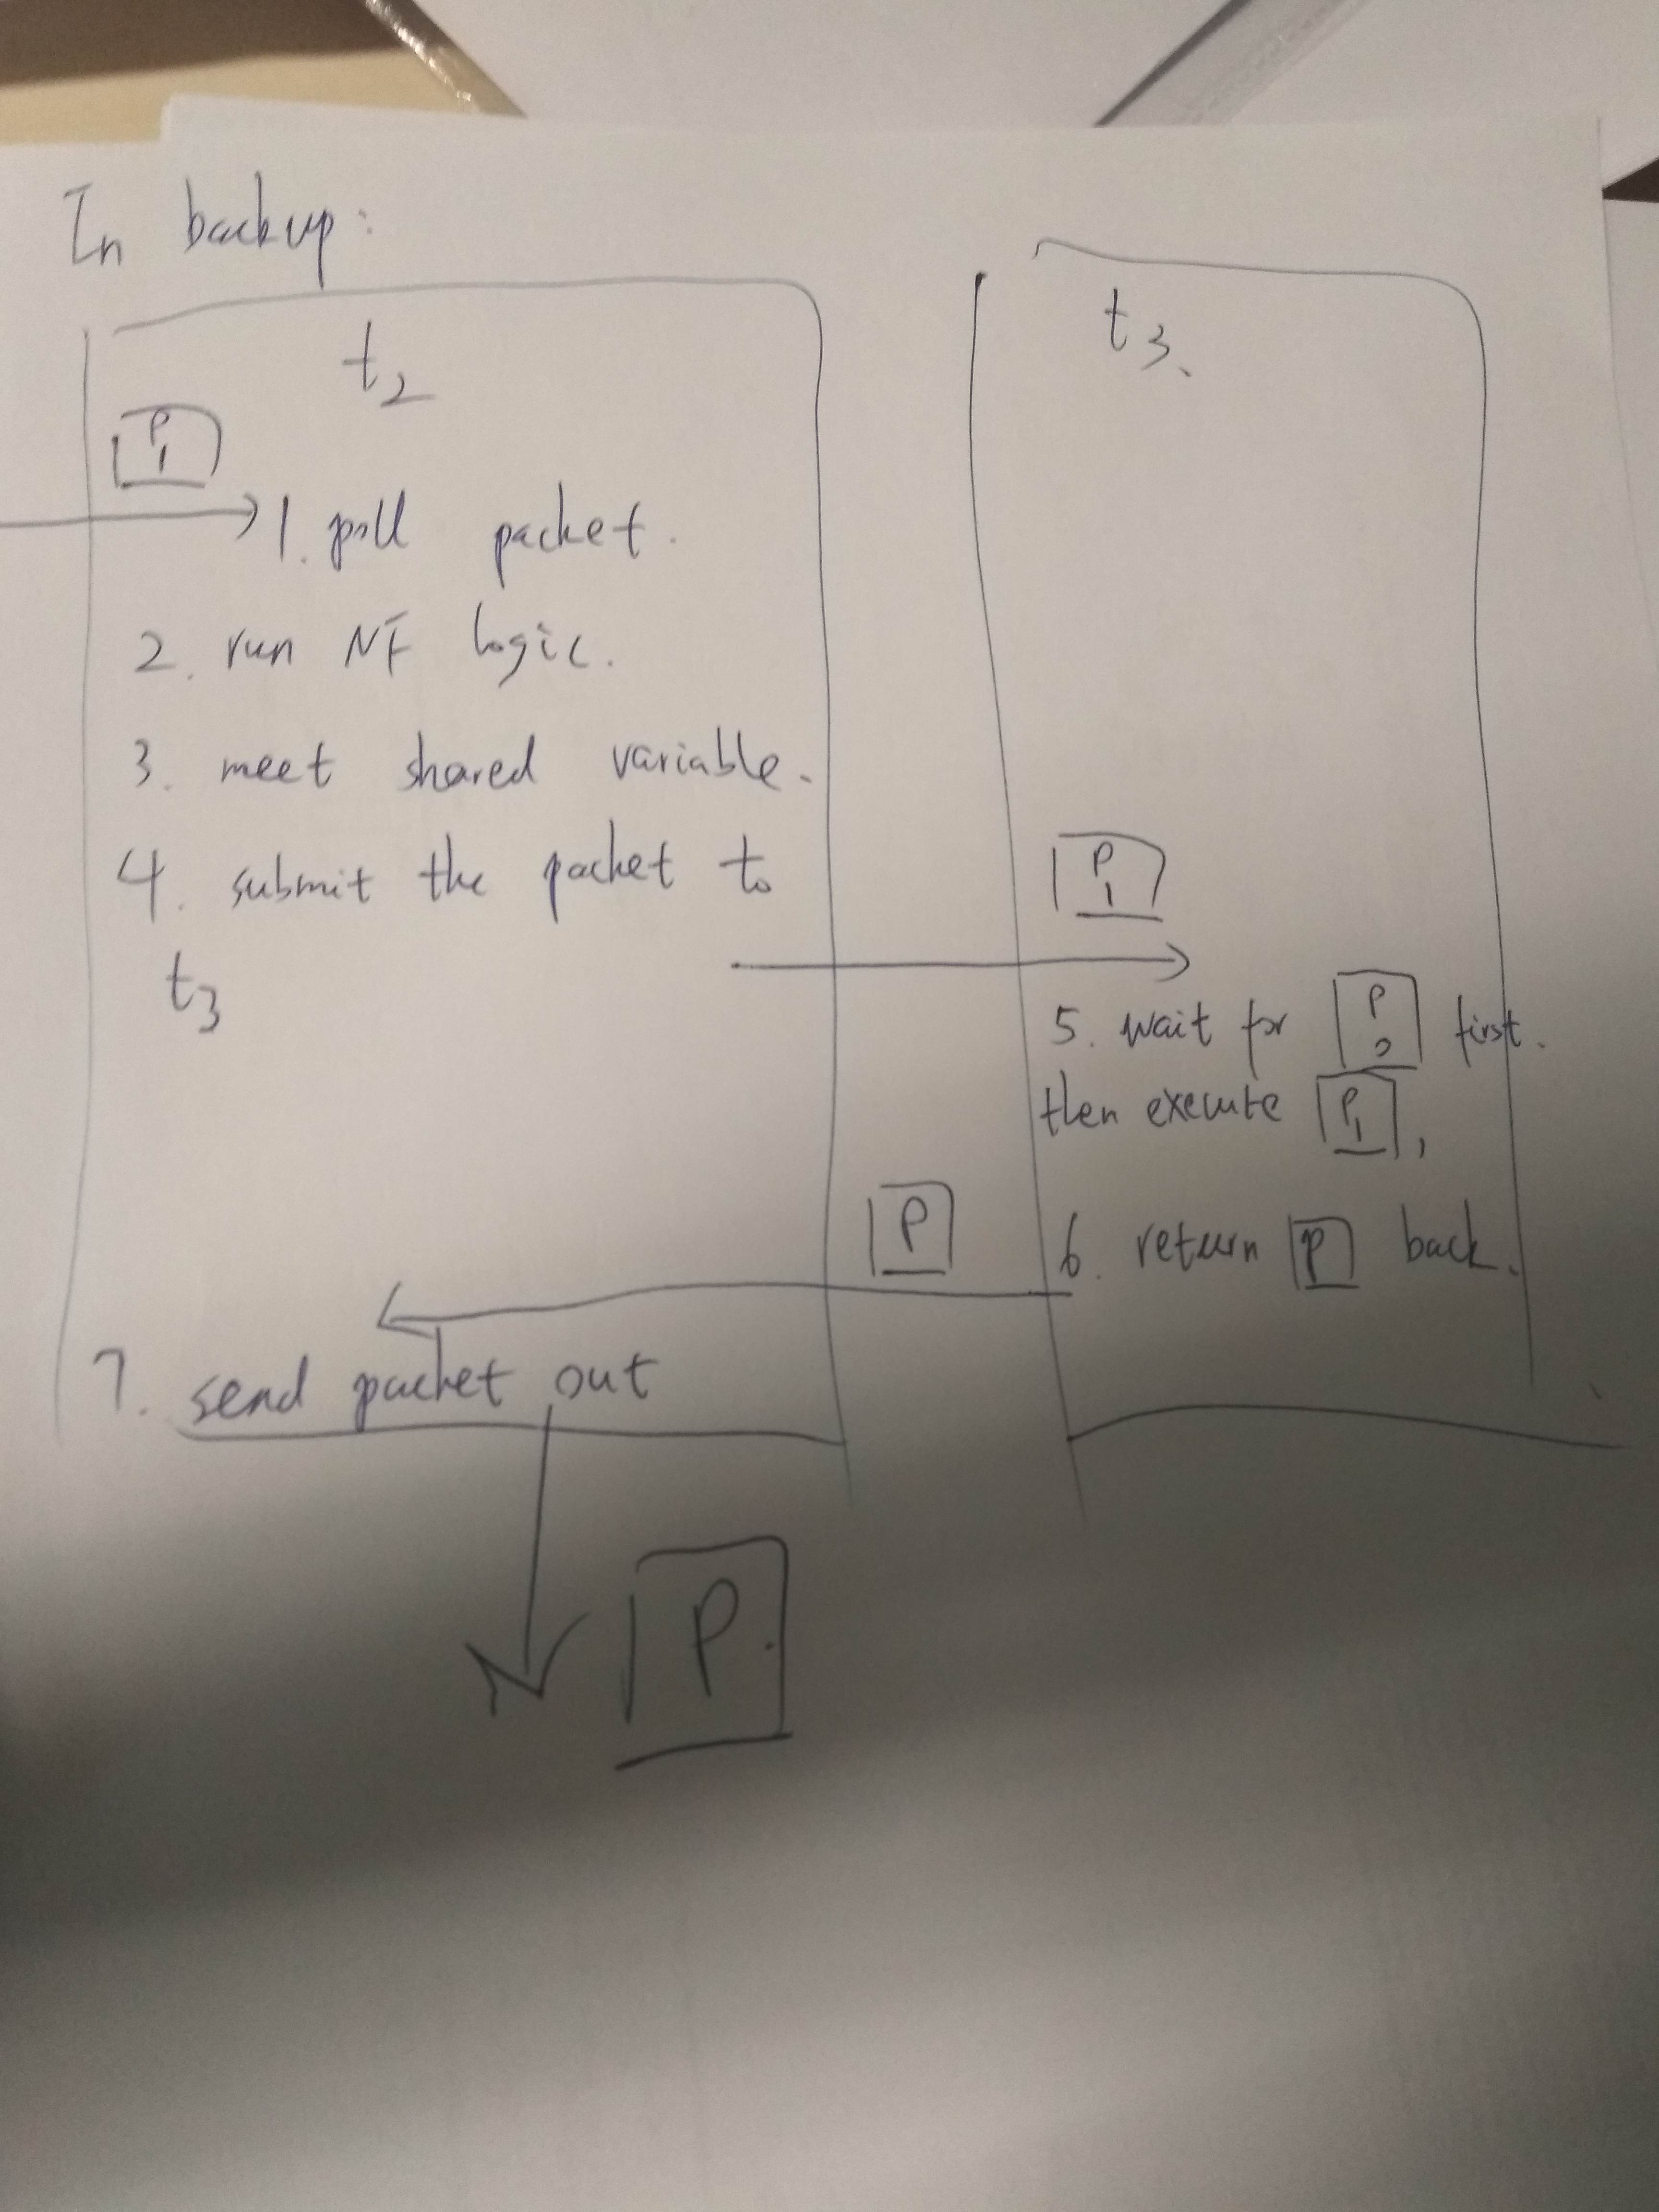
\includegraphics[width=\columnwidth]{section/backup.jpg}
    \resizebox{0.95\columnwidth}{!}{\theverbbox}
    \caption{The execution flow on a backup instance.}\label{fig:backup}
  \end{subfigure}
%Removed for better illustration.
\caption{Work flow of how to keep both primary and backup in synchronization.}
\label{fig:fig}
\end{figure}

\subsection{Basic Setup for Recovery without Rolling Back}

The basic setup is shown in figure \ref{fig:overall}. We set up two identical NF
instances. The two instances run the same NF software binary image and are
configured with the same number of CPU cores.

In \ref{fig:overall}, the NF instance is configured with two worker threads
($t_1$ and $t_2$) which poll the NIC card for input packet. The shared variable
is hosted on a dedicated thread $t_3$.

To access the shared variable hosted on $t_3$, both $t_1$ and $t_2$ need to send
a message for accessing the shared variable to $t_3$. After the shared variable
is modified, another message is sent back to $t_1$ or $t_2$ to indicate the
completion of shared variable modification.

When the primary instance finishes processing the input packet, it forwards the
input packet to the backup instance over a reliable communication channel. The
backup instance processes the input packet again before releasing the
packet. The packet processed by the backup instance is tagged with an execution
order by the primary, so that the shared variable on the backup instance can
process the input packet in the same sequence as the primary instance. This
guarantees that the state of both the primary instance and the backup instance
are always synchronized.

\subsection{Workflow on Primary Instance}

Figure \ref{fig:primary} shows how worker thread $t_2$ processes an input
packet. The overall workflow is similar to a typical packet polling loop. The
only exception is that when a shared variable is going to be accessed by $t_2$
(step 3 in figure \ref{fig:primary}), instead of directly acquiring the lock and
update the shared variable, $t_2$ sends the packet to $t_3$ to update the shared
variabale (step 4). When $t_3$ receives this packet, the threads update the
shared variable (step 5), tags the packet with a sequence number (step 6) and
sends the packet back to $t_2$. When $t_2$ receives this packet, $t_2$ sends the
tagged packet out to the backup instance over a reliable communication channel.

\subsubsection{The Sequence Number}

The sequence number tagged by $t_3$ indicates a sequential accessing order to
the shared variable. Using this sequence number, the backup instance can
reliably reproduce the accessing order of the shared variable (to be discussed
in section \ref{sec:backup}). This ensures that the state of the primary and backup
instances are always synchronized.

\subsubsection{Using Future and Promise to Cancel Thread Blocking}

The biggest problem with this workflow is that, after step 4 in figure
\ref{fig:primary}, worker thread $t_2$ must block its execution and wait for the
packet to come back from $t_3$. This is unacceptable for a high-performance NF
software.

We tackle this problem using futures and promises in reactive
programming. After step 4 in figure \ref{fig:primary} is executed, we wrap the
current thread context inside a future object. $t_2$ can immediately start processing
other input packets. When the packet comes back to $t_2$ after step
6, $t_2$ is able to re-construct the previous thread context using the
corresponding future object. This efficiently eliminates thread blocking.

\subsubsection{The Reliable Communication Channel}

Due to the power of future and promise, a user-space TCP/IP stack could be
integrated inside $t_2$. The reliable communication channel is actually a TCP
connection channel. This reliable communication channel is augmented with flow
control and is more reliable than other specially-crafted reliable communication protocols. 

\subsection {Workflow on Backup Instance}
\label{sec:backup}

Figure \ref{fig:backup} shows how worker thread $t_2$ processes the output
packet sent from the primary instance. The overall workflow is similar to that
of the primary instance. However, when the packet is delivered to $t_3$ to
access the shared variable, $t_3$ must check whether it has processed all the
packets whose sequence number is smaller than the packet. Considering the case
of figure \ref{fig:backup}, $t_3$ must wait for packet with sequence number 0
first. If $t_3$ has processed packet with sequence number 0, $t_3$ can directly
process the packet with sequence number 1. Otherwise, $t_3$ should store packet with
sequnece number 1 and wait for the packet with sequenece number 0 to come.

Since the order of how packets access the shared variable is well preserved,
the backup instance and the primary instance have the same state.

\subsection{Recovery}

If the primary instance fails, the backup instance can become the primary
instance immediately. The recovery time is basically decreased to zero.





